% !TeX program = lualatex

\documentclass[12pt]{report}
\usepackage[Glenn]{fncychap}
\usepackage[T1]{fontenc}
\usepackage[francais]{babel}
\usepackage{fontspec}
\usepackage{wrapfig}
\usepackage{graphicx}
\usepackage{soul}
\usepackage[colorlinks=true, linkcolor=black, urlcolor=black, citecolor=black]{hyperref}
% \usepackage[hyphens, spaces, obeyspaces]{url}
\usepackage[a4paper, width=175mm, top=25mm, bottom=25mm]{geometry}
\usepackage{parskip}
\usepackage{enumitem}
\usepackage{titlesec}
\usepackage{listings}
\usepackage{float}
\usepackage[final]{pdfpages}
\usepackage{xcolor}
\usepackage{tocbibind}
\usepackage{tocloft}
\usepackage{xpatch}
\usepackage{amsmath}
\usepackage{amsthm}
\usepackage{amsfonts}
\usepackage{graphics}
\usepackage{color}
% \usepackage[grey,utopia]{quotchap}
\usepackage{moreverb}
\usepackage{xcolor}
\usepackage{framed}
\usepackage{arabluatex}
%\usepackage[algo2e, french, onelanguage, ruled]{algorithm2e}
\setlist[itemize]{label=\textbullet}
\usepackage{fancyhdr}
\pagestyle{fancy}   
\fancyhead{}
\fancyhead[C]{\leftmark}
\renewcommand{\headrulewidth}{0.4pt}
\renewcommand{\footrulewidth}{0.4pt}
\usepackage{xcolor}
\definecolor{light-gray}{gray}{0.90}
\usepackage{multirow}
\usepackage{soul}
\usepackage{graphicx}
\usepackage[utf8x]{inputenc}
\setcounter{secnumdepth}{3} 
\usepackage{dirtytalk}
\usepackage{csquotes}

\begin{document}

%\title{Réalisation d'un assistant virtuel intelligent pour ordinateurs}
%\author{W.Benhaddad, Y.Bourahla}
\date{2018}

\tableofcontents

\chapter*{Introduction générale}
\begin{itemize}
	\item Ici on parlera des motivations qui ont aboutis à ce projet, des objectifs de ce dernier ainsi que ses perspectives
\end{itemize}


\chapter{Assistants virtuels intelligents}

\section{Introduction}
\paragraph{}
Depuis la commercialisation du premier ordinateur grand public (Xerox PARC Alto) en 1973, le monde découvrit pour la première fois ce qui allait devenir l'apparence basique de chaque ordinateur moderne. En effet, la compagnie Xerox fut la première à proposer une interface graphique dotée de fenêtres, d'icônes et d'une souris pour se déplacer et d'un clavier pour écrire du texte. Bien que basique, cette idée lança alors plusieurs autres grandes marques sur le même chemin (IBM, Apple, Compaq ...). Par la suite, beaucoup ont essayé d'améliorer la façon dont l'homme utilisait sa machine : souris plus précise, écran doté d'une plus grande résolution, clavier plus enrichi, voire même l'introduction des écrans tactiles dans certains systèmes embarqués.
\par Cependant, certains voyaient encore cette façon d'utiliser la machine comme trop primitive, et peu intuitive. En effet laissez un enfant devant un ordinateur et il prendrait un bon moment pour apprendre à éditer ne serait ce qu'un simple fichier. Pour citer Donald A. Norman :
\begin{quote}
	\say{We must design for the way people behave, not for how we would wish them to behave.}\cite{don-norman}
\end{quote}
que nous pouvons traduire par :
\begin{quote}
	\say{Nous devons concevoir selon le comportement des utilisateurs, et non pas selon la façon dont nous voudrions qu'ils se comportent.}
\end{quote} 
L'humanité a fait beaucoup de chemin depuis les années 70, l'utilisation d'un ordinateur de nos jours avec les moyens classiques (souris, clavier, écran ...) est devenue une tâche triviale, voire même une \textcolor{red}{seconde nature, cela reste cependant dû au fait que de plus en plus de jeunes enfants sont exposés depuis leur plus jeune âge au monde technologique qui les entoure, le processus d'apprentissage reste cependant présent, l'effort d'utiliser les outils communs reste lui aussi présent.}
\par La plus naturelle et plus ancienne façon de communiquer pour l'homme a toujours été la parole. Le développement de langues toutes aussi riches et complexes les unes que les autres a permis à l'humanité de briser plusieurs \textcolor{blue}{barrières sociales}. L'avancement le plus naturel pour cette façon de communiquer serait donc de l'étendre aux machines que l'homme a su construire et améliorer au fil des années.
\par 
Motivé par cette manière que l'on a de communiquer entre nous, et épaulé par les récentes technologies telles que l'apprentissage automatique, le traitement automatique du langage naturel et l'intelligence artificielle, les plus brillants des chercheurs ont entamé leurs travaux dans cette toute nouvelle direction.
\par 
Les Assistants Virtuels Intelligents (Smart Personal Assistant, SPA \cite{SPA-overview}) sont donc le produit de plusieurs années de recherche, visant tout d'abord à faciliter certaines tâches pour l'utilisateur. Les premiers SPAs étaient conçus comme des agents de conversation ou Chatbots, limités dans leurs actions et dépendant toujours d'un moyen de communication textuel, ce n'était pas la forme désirée du SPA. Avec l'avancement des recherches sur la reconnaissance automatique de la parole (Automatic Speech Recognition, ASR) et l'émergence de l'apprentissage automatique, les tout premiers assistants virtuels utilisant l'ASR étaient spécialisés dans certains domaines comme des systèmes médicaux d'aide à la décision. Il a ensuite été plus aisé de briser la barrière et de réaliser ce qui était encore une esquisse d'un SPA personnalisé. Aujourd'hui, et ce depuis l'avènement de l'apprentissage profond et la popularisation des Smartphones, de nouveaux SPAs comme Apple Siri (voir \ref{siri}) et Google assistant (voir \ref{googleass}) et Amazon Alexa (voir \ref{alexa}) ont fait leurs apparitions, offrant de plus en plus de services personnalisés et spécifiques à chaque utilisateurs.
\par 

Dans la suite de ce chapitre nous essayerons de mieux détailler ce qu'est un SPA, ce qui est demandé d'un tel système, ses domaines d'application, en enchaînant par une description d'une pseudo-architecture potentielle de ce système, pour enfin  conclure sur les limitations actuelles et les motivations de ce projet. 

\newpage
\section{\textcolor{red}{L'importance du contexte pour un SPA}}\label{spa-def}
Informellement, un SPA est un type d'agent (voir \ref{agent}) logiciel qui peut effectuer certaines tâches et proposer des services dédiés aux utilisateurs qui vont d'une simple tâche (Ouvrir une fenêtre, lancer une application ...) à la réalisation de requêtes un peu plus complexes comme réserver une table dans un restaurant en passant un appel vocal (voir \ref{duplex}). Pour répondre efficacement à toutes sortes de requêtes, un SPA se doit donc de garder trace du contexte courant de sa conversation avec l'utilisateur. Il doit disposer d'un système capable d'enregistrer les informations pertinentes et de savoir les réutiliser, mais aussi de pouvoir déduire lesquelles de ces informations sont manquantes. On parle ici de Context-Awarness ou Sensibilité au contexte, comme vu dans \cite{SPA-overview}.
\par D'après \cite{SPA-overview} et \cite{Dey-Abwod},
\textit{Day} et \textit{Abwod} définissent un contexte comme suit : 
\begin{quote}\label{context-def}
	\say{A context is any information
		that can be used to characterize the situation of an entity. An entity is a person, place,
		or object that is considered relevant to the interaction between a user and an
		application, including the user and applications themselves}
\end{quote}
qui peut être traduit par :
\begin{quote}\label{context-def-fr}
	\say{Un contexte est une information qui peut être utilisé pour caractériser l'état d'une entité. Une entité peut être une personne une place ou un objet, considérée comme pertinente à  l'interraction entre l'utilisateur et l'application, ainsi qu'à ces deux derniers eux mêmes}
\end{quote}
Il en découle que pour parvenir à développer un système qui puisse répondre aux besoins individuels et spécifiques de chaque personne, modéliser et prendre en compte le contexte semble être une solution prometteuse.



\section{Caractéristiques principales d'un SPA}
\paragraph{}
À partir de \cite{SPA-overview}, nous pouvons dégager certaines caractéristiques principales qui peuvent être vues comme primordiales pour qualifier un assistant virtuel comme étant intelligent.
\subsection{Sensible au contexte}
\paragraph{}
Comme précédemment vu dans la définition du contexte (section \ref{context-def}), ce dernier peut être interprété comme tout aspect d'une entité (position d'un objet, couleur d'un objet, température d'une chambre, etc.). Un assistant dit intelligent doit donc être capable de capturer le concept du contexte, d'utiliser et de traiter toute information catégorisée comme contextuelle.
Pour être plus précis, un SPA doit être sensible à l'évolution du contexte courant, par le biais de capteurs optiques, de microphones, ou tout ce qui pourrait amener l'utilisateur à faire évoluer la requête qu'il a émise. L'assistant devra donc proposer un système de mise à jour du contexte pour éliminer les informations inutiles et garder celles qui pourraient aider à répondre à la requête de l'utilisateur.
\subsection{Évolutif}
\paragraph{}
Comme vu dans la section \ref{spa-def}, un SPA peut être vu comme un type d'agent. Pour rappel, d'après \textit{Russel} et \textit{Norvig} dans \cite{RussellAgent}, un agent\label{agent} est une entité autonome pouvant interagir avec son environnement afin d'accomplir certaines tâches et peut être de plusieurs types : 
\begin{itemize}
	\item Agent à réflexes simples : agent exécutant ses actions à base de règles conditionnelles simples (c.à.d Si \textit{Condition } alors \textit{exécuter actions}), ils sont ainsi très simplistes et limités dans la portée de leurs actions.
	
	\item Agent basé modèle : semblable aux agents à réflexes simples, il est doté d'un modèle interne complexe censé représenter le monde extérieur auquel l'agent a accès. Cependant, il applique les actions de la même manière que le précédent type d'agents.
	
	\item Agent à but : ce type représente une amélioration des agents simples puisqu'il est doté d'un ensembles d'états buts à atteindre d'une façon ou d'une autre.
	
	\item Agent à utilité : il s'agit ici agents à buts qui tentent d'aboutir à leurs buts d'une manières optimisée (intelligente) utilisant une fonction de mesure adéquate pour le choix des différents états à atteindre.
	
	\item Agent apprenant : agent à utilité enrichi par un module d'apprentissage qui sert de juge pour répondre aux "critiques" des actions qu'il entreprend. Le terme agent évolutif est aussi employé.
\end{itemize}
\par Pour ce qui est des SPAs, les plus récents systèmes (ex : Amazon Alexa qui améliore son  module de reconnaissance de la parole après chaque réponse non \textcolor{blue}{réfutée} par l'utilisateur) peuvent être considérés comme des agents apprenants, répondant de ce fait à la contrainte évolutive imposée. Cependant, le domaine de l'auto-évolution des systèmes intelligents est encore un domaine nouveau qui se voit \textcolor{blue}{aidé} par les récentes avancées dans l'apprentissage automatique \cite{SPA-overview}.


\subsection{Multimodal}
\paragraph{}
Afin d'assurer une aisance d'utilisation, les SPAs sont fréquemment amenés à récupérer les requêtes (ou données) en entrée de la manière la plus naturelle possible (par exemple par le biais de la parole). Cependant, pour garantir une expérience d'utilisation adéquate, l'assistant sera souvent confronté à récupérer ces requêtes de différentes manières, que ce soit à travers une interface graphique (écran tactile) ou à travers un texte brut tapé au clavier, voire même à travers des expressions faciales ou des états cognitives/émotionnels \cite{Dingler2016}, pour ensuite produire une réponse qui elle aussi pourrait éventuellement être de la forme textuelle, sonore ou les deux. Cette capacité à recevoir en entrée et/ou produire une sortie de plusieurs façons différentes est appelée la multi-modalité \cite{Luger2016}. Cette caractéristique permet de masquer à l'utilisateur toute la complexité d'acquisition de ses requêtes.

\subsection{Anthropomorphe}\label{antropo}
\paragraph{}
Plusieurs auteurs tendent à attribuer une grande importance à l'anthropomorphisme des SPAs \cite{virtualbutler}, qui est 
\begin{quote}
	\say{Un mécanisme qui pousse les êtres humains à induire qu'une entité non-humanoïde possède des caractéristiques et comportements propres à l'homme}\cite{alexabff}
\end{quote}

\par Ce comportement humanoïde pousserait donc l'utilisateur à se sentir plus à l'aise avec l'assistant, le conduisant ainsi à adopter une façon de communiquer plus humaine et moins structurée qu'avec les autres machines. Ceci est une caractéristique majeure d'un SPA se disant personnalisé.
\subsection{Multi-plateforme et Flexible }
\paragraph{}
Malgré leurs récentes prouesses, certains SPAs sont encore restreints à un écosystème fortement dépendant du fabricant.  Cowan et al. mentionnent dans \cite{Cowan2017} que Apple Siri est limité à l'environnement constitué des produits de la firme à la pomme, n'ouvrant par défaut que les applications de cette dernière quand une requête lui est transmise. C'est un comportement que les assistants devraient éviter, car une indépendance des plateformes utilisées est, certes, très complexe à instaurer, mais offre plus de possibilités aux utilisateurs et aux développeurs pouvant ainsi exploiter la puissance de certaines plateformes (Smartphones, TV connectées, etc).
Avec l'émergence de l'IoT (Internet of Things) et des maisons intelligentes  par exemple, c'est un tout nouveau terrain de jeu qui est présenté aux SPAs, offrant plus d'opportunités pour les utilisateurs.
\section{Domaines d'applications des SPAs}
\paragraph{}
Après avoir vu les différents aspects que les SPAS doivent traiter, nous nous intéresserons maintenant aux types de services et applications que ces derniers pourraient fournir pour démontrer qu'ils peuvent bel et bien faciliter certaines tâches à l'homme.

\subsection{Vie quotidienne}
\paragraph{}
À la base, les SPAs étaient destinés à un usage très personnel comme la gestion des achats dans les supermarchés, ou des guides touristiques de plusieurs destinations de voyage. Cette spécificité a commencé à s'estomper petit à petit avec l'émergence de nouveaux systèmes dédiés à des applications plus générales, comme les maisons intelligentes ou les assistants de planification de tâches. Ceci a permit de mettre encore plus l'accent sur cet aspect de convivialité que les tout premiers SPAs ont tenté de perfectionner. Ainsi, ces assistants spécialisés dans des domaines restreints (Tourisme, shopping, détente, etc) ont été regroupés dans un seul système plus polyvalent, capable de répondre à des besoins quotidiens divers et variés, allant même à fournir une assistance aux personnes âgées pour leur faciliter les tâches rudimentaires devenues trop fatigantes. 
\subsection{Assistance professionnel}
\paragraph{}
Les SPAs ont aussi une place dans le monde professionnel. Dans \cite{Imtiaz2014} il est cité que dans les situations où la marge d'erreur est très petite (par exemple dans les système de manufacturing \footnote{Manufacturing ici dans le sens chaîne de montage industrielle, par exemple dans des usines.}) l'assistance d'un SPA est nécessaire servant d'extension au cerveau humain pour l'aide à la décision.
\par
Par exemple, dans un environnement de travail hétérogène (Nouveaux/anciens employés, Hiérarchies des postes ...) les SPAs pourraient délaisser les employés les plus expérimentés de la tâche d'assister les nouveaux arrivants, pour ainsi aider ces derniers dans leurs tâches et permettre aux autres de se focaliser sur les leurs.

\subsection{E-Apprentissage}
\paragraph{}
Les SPAs peuvent aussi être utiles dans l'enseignement, aussi  bien dans un milieu académique que professionnel. D'une part ils pourraient occuper plusieurs rôles dans les établissements scolaires (correcteur automatique de copies, enseignant interactif ... ). \cite{ENGAGINGTA}, et d'autre part accompagner les employés durant leurs formations professionnelles.
\par
Ainsi en considérant les caractéristiques d'un SPA, la sensibilité au contexte est reliée aux expériences antérieures de l'apprenant permettant au SPA d'adapter son processus d'enseignement en conséquence.\par  En ce qui concerne l'aspect évolutif du SPA, il lui  de favoriser une approche d'enseignement à une autre selon les résultats de ses apprenants.

\newpage
\section{Exemples de SPAs}
\paragraph{}
Pour illustrer la puissance des SPAs les plus récents, nous avons décidé de mettre en évidence les quatre produits qui dominent le marché courant :

\subsection*{Google assistant}\label{googleass}
\paragraph{}
\begin{figure}[H]
	\centering
	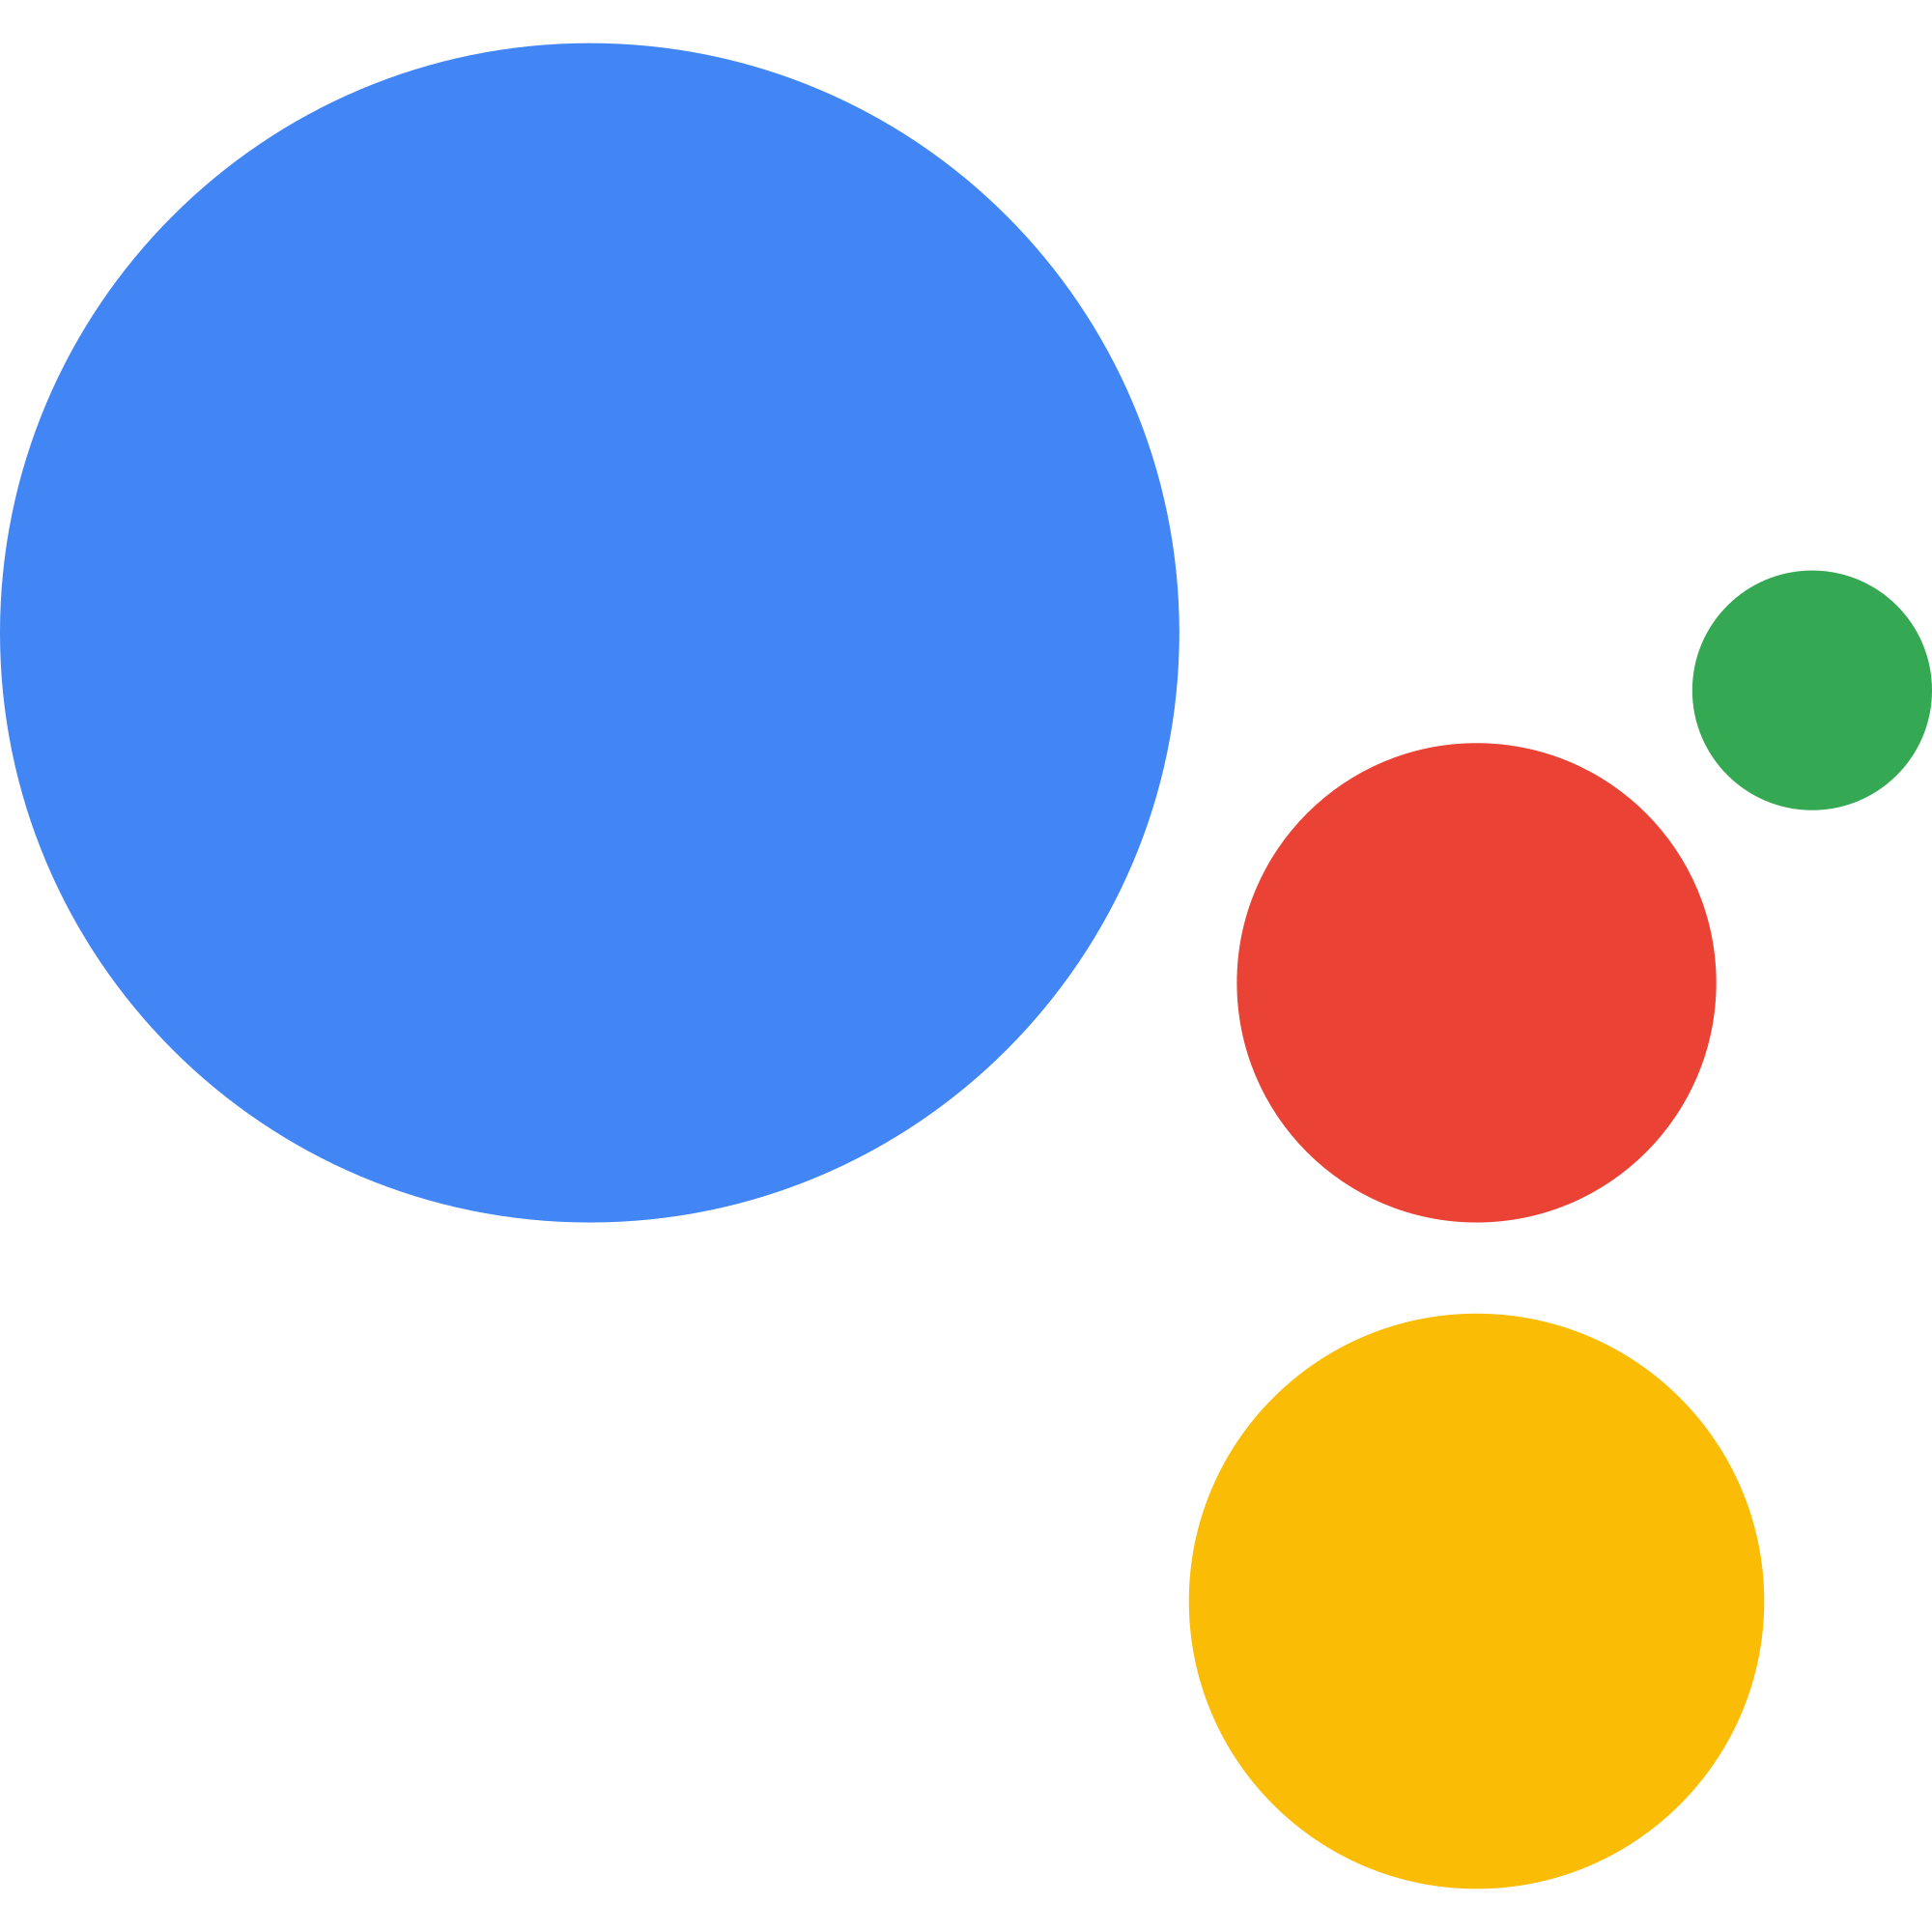
\includegraphics[width=.2\linewidth]{images/google_assitant/logo.png}
	\caption{Logo de Google assistant} 
\end{figure}
Lancé en 2016 comme un chatbot(\ref{chatbot})intégré dans l'application Google Allo,  Google Assistant (G.A) s'est vu ensuite être directement intégré sur les système d'exploitation Android(que ce soit sur smartphones ou tablettes, et plus récemment sur Google Home\footnote{Appareil servant à contrôler les composant d'une smart-house ainsi que l'utilisation des différents services de google}). G.A est un assistant à tout faire concocter par les ingénieurs de Google dans le but de faciliter la recherche sur internet, la planification des tâches, l'ajustement des réglages de l'appareil ..., son point fort est sa capacité à engager une conversation bi-directionnel avec l'utilisateur, assurant ainsi une interaction personnalisé variant d'un utilisateur à un autre, cela lui permet par exemple de proposer certains résultats de recherche selon les précédentes interactions avec l'utilisateur ou de lui proposer une activité si ce dernier lui reproche de s'ennuyer(voir figure \ref{boredpic}).
\begin{figure}[H] 
	\label{boredpic} 
	\centering
	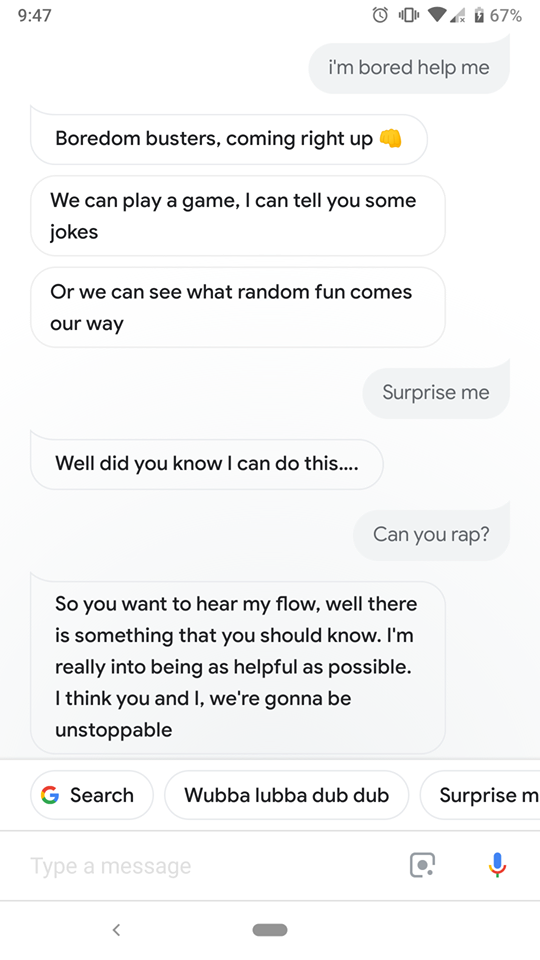
\includegraphics[width=.5\linewidth]{images/google_assitant/bored.png} 
	\caption{Conversation aléatoire avec G.A} 
\end{figure}

\begin{figure}[H]
	\centering
	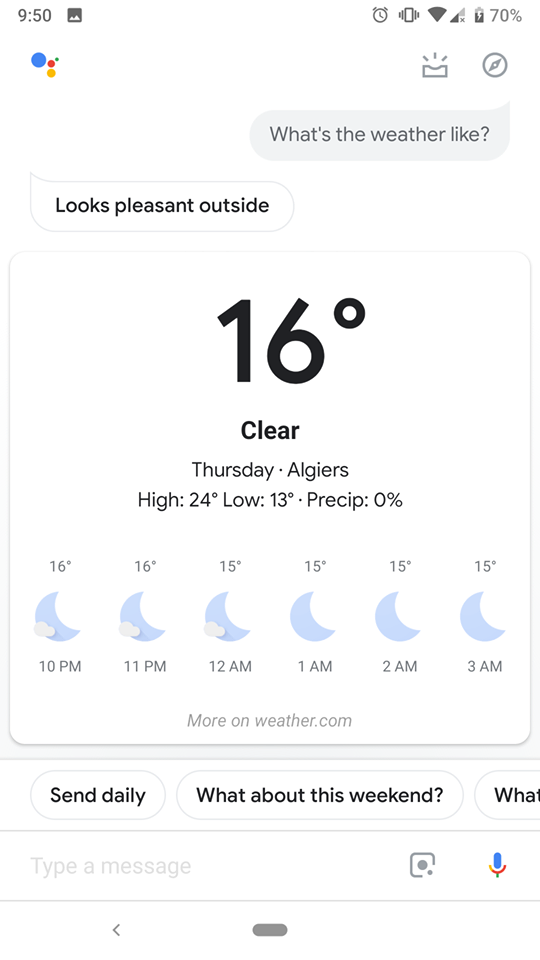
\includegraphics[width=.5\linewidth]{images/google_assitant/weather.png} 
	\caption{Requête simple formulée à G.A} 
	
\end{figure} 


\subsubsection*{Google duplex}\label{duplex}
\begin{figure}[H]
	\centering
	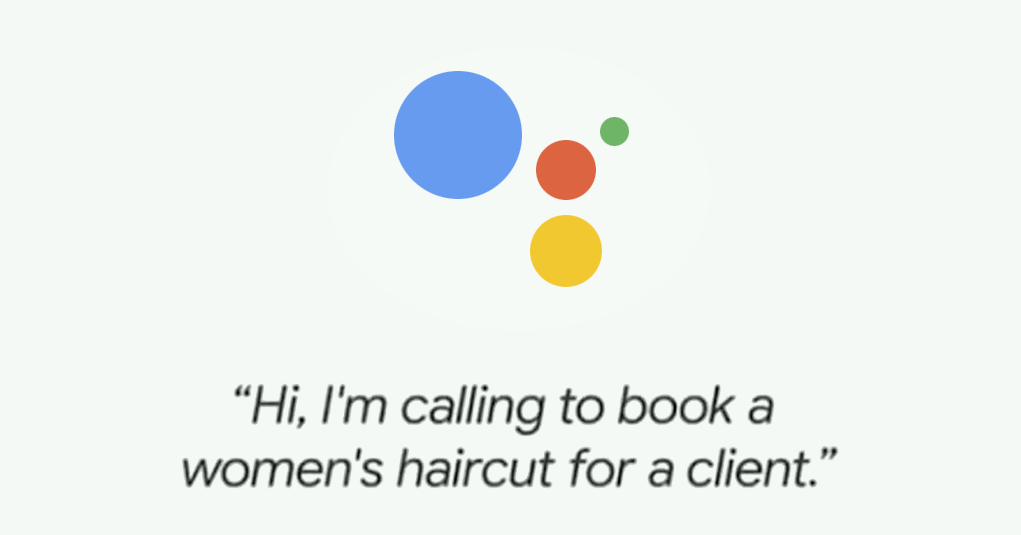
\includegraphics[width=.5\linewidth]{images/google_assitant/duplex.png} 
	\caption{Google duplex en réservant une place dans un salon de coiffure} 
\end{figure}
\par Une des nouveautés impressionnante de G.A est la fonctionnalité Google Duplex, toujours en phase de développement, ce module est capable de passer des appels a de vrais personnes et d'avoir une conversation avec elles afin de réaliser une tâche demandée par l'utilisateur comme par exemple réserver une chambre d'hôtel, une table au restaurant ... 



\subsection*{Apple Siri}\label{siri}
\begin{figure}[H]
	\centering
	
\includegraphics[width=.25\linewidth]{images/apple_siri/logo.png}
	\caption{Logo d'Apple Siri} 
\end{figure}
\paragraph{}
Siri est l'assistant virtuel développé par Apple, contrairement aux SPAs durant sa sortie, Siri proposait une nouvelle façon de communiquer avec l'utilisateur, à travers une interface de requêtes vocale, et une façon de communiquer très humanoïde (satisfaisant ainsi le critère d'anthropomorphisme voir \ref{antropo}).
Siri est capable de répondre à des questions précises(voir figure \ref{macbooksiri}), de proposer des recommandations, déléguer la requête à des services web ou d'autres application (voir figure \ref{whatsapp} et \ref{cashconfirm}). Il a l'avantage(et l'inconvénient) d'être disponible sur la multitude d'appareils qui composent l'écosystème d'Apple (MacBook,iPhone,iWatch ...).

\begin{figure}[H] 
		\centering
		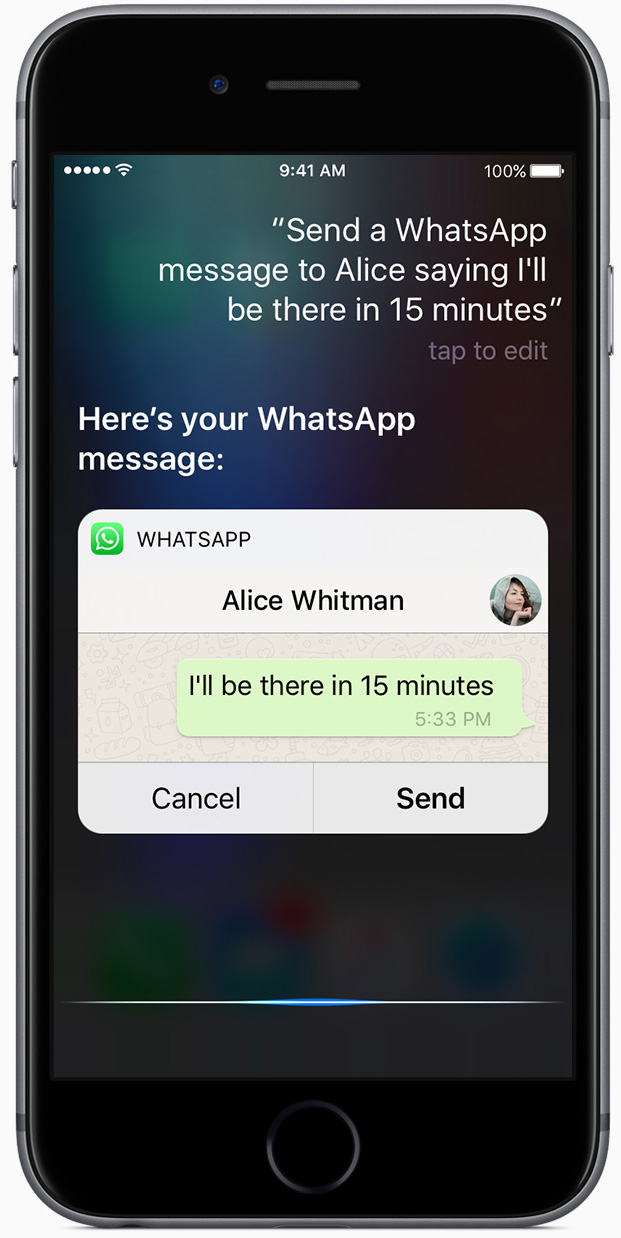
\includegraphics[width=.25\linewidth]{images/apple_siri/whatsapp.jpg} 
		\caption{Intégration aux applications \cite{siriDemo}}
		\label{whatsapp}
\end{figure}

\begin{figure}[H]
	\centering
	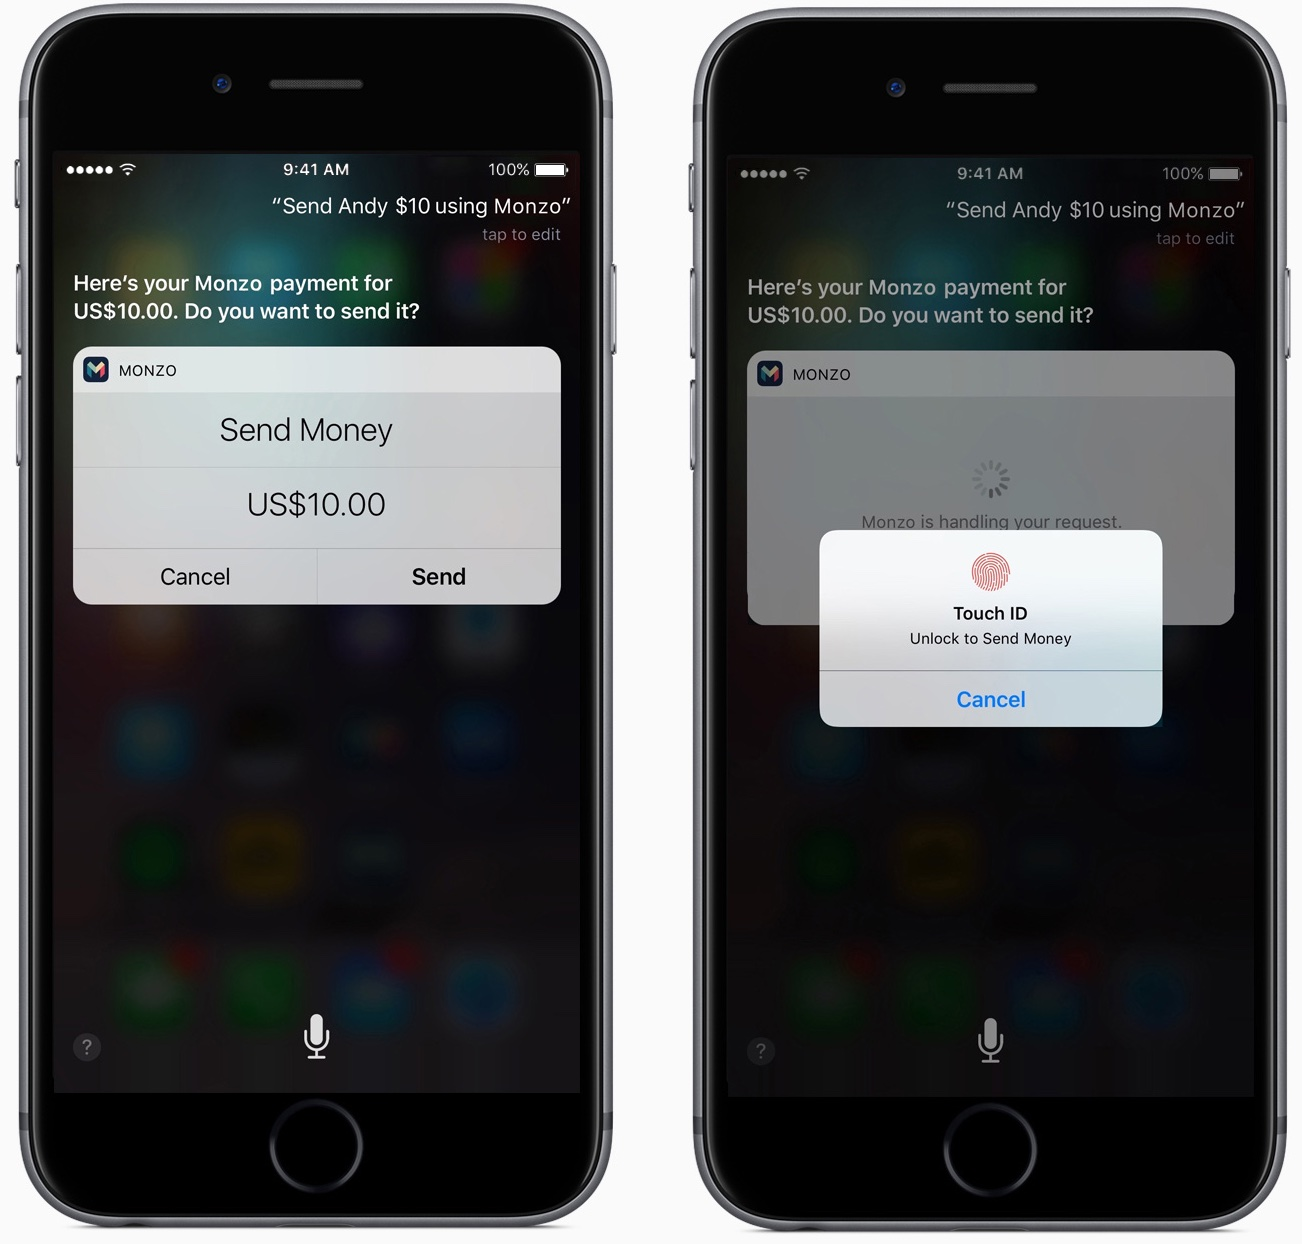
\includegraphics[width=0.5\linewidth]{images/apple_siri/cashconfirm.jpg} 
	\caption{Service paiement 1 \cite{siriDemo}}
	\label{cashconfirm}
\end{figure}

\begin{figure}[H]
	\centering
	\label{macbooksiri}
	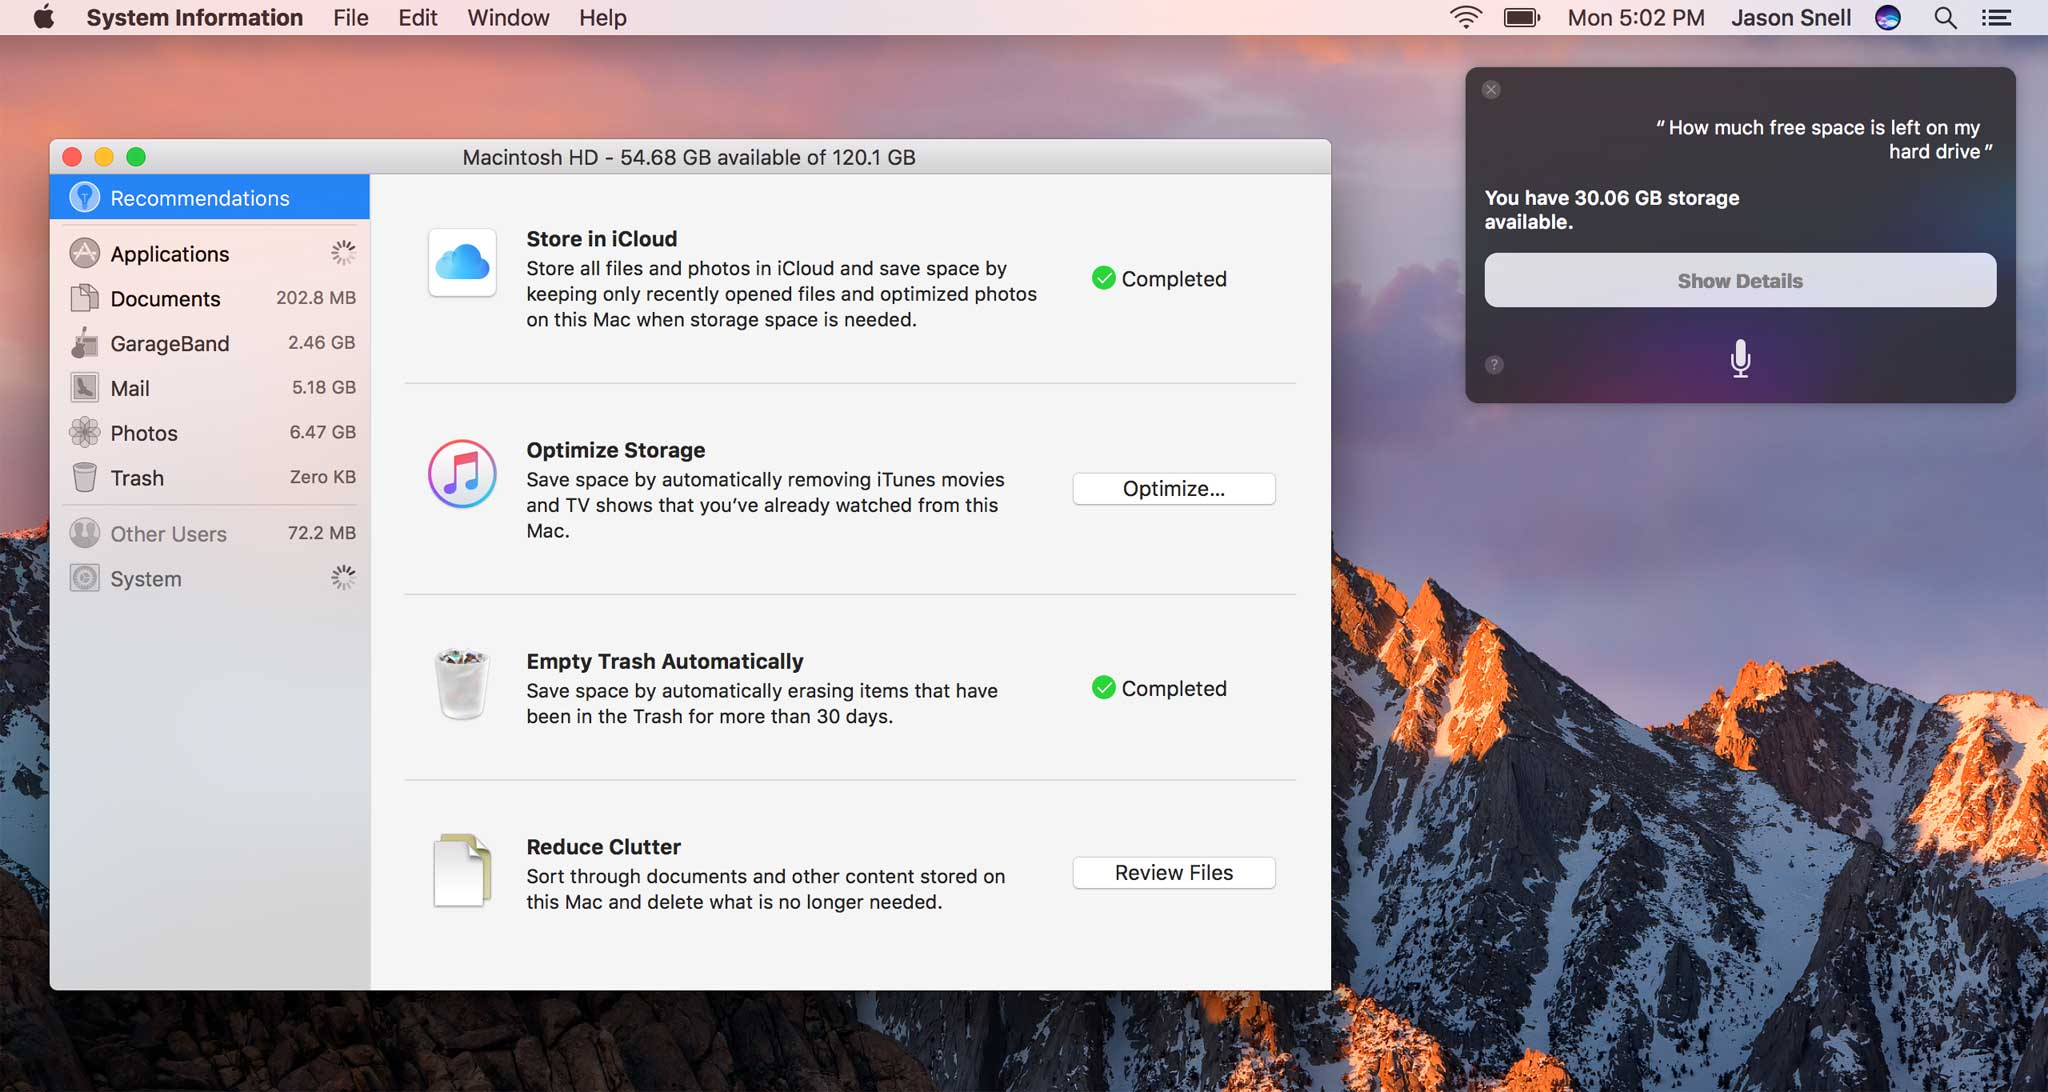
\includegraphics[width=0.75\linewidth]{images/apple_siri/macbook.png} 
	\caption{Siri sur un laptop  \cite{macossiridemo}}
\end{figure}


\subsection*{Amazon Alexa}\label{alexa}
\begin{figure}[H]
	\centering
	
\includegraphics[width=.5\linewidth]{images/amazon_alexa/logo.png}
	\caption{Logo d'Amazon Alexa} 
\end{figure}
\paragraph{}Amazon Alexa est un assistant exclusivement intégré au dispositif Amazon Echo(un haut-parleur portatif), à l'instar de Siri, il est aussi capable de communiquer avec l'utilisateur par le biais de la parole, pouvant ainsi exécuter diverse commandes comme jouer de la musique, réciter des livres audios, annoncer des news en temps réel (Résultats sportifs, tendances politiques ... ). Son atout majeur est sa capacité à s'intégrer à plusieurs appareils-connectés (Contrôleur de thermostat ou de lumières ambiantes dans une Smart-House ) ainsi que la possibilité d'ajout des SKILLS (ou compétences) de la part des développeurs tiers pour enrichir la panoplie de services que peut offrir Alexa.
\begin{figure}[H]
	\centering
	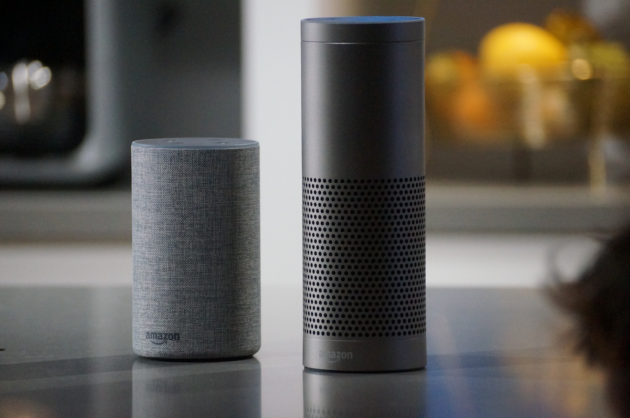
\includegraphics[width=.75\linewidth]{images/amazon_alexa/alexa.png}
	\caption{Haut parleur Echo embarquant le SPA Alexa} 
\end{figure}
\subsection*{Microsoft Cortana}
\begin{figure}[H]
	\centering
	
\includegraphics[width=.5\linewidth]{images/cortana/logo.png}
	\caption{Logo de Microsoft Cortana} 
\end{figure}
\paragraph{}
Cortana est la tentative de la part de Microsoft d'intégrer un assistant dans son système d'exploitation Windows 10 et WindowsPhone,. Il propose divers services de base tel que planifier des tâches, exécuter des commandes via la parole, et analyser des résultats de recherche sur le moteur de recherche de Microsoft, à savoir Bing, pour répondre à des questions.
\begin{figure}[H]
	\centering
	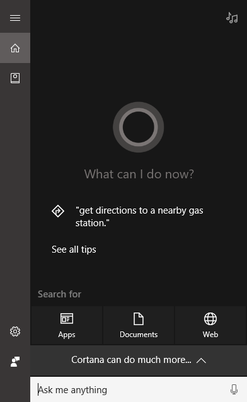
\includegraphics[width=.4\linewidth]{images/cortana/weather.png}
	\caption{Cortana répondant à une requête utilisant Bing } 
\end{figure}

\section{Architecture générale d'un SPA}
\paragraph{}
Il n'existe pas vraiment d'architecture type pour un SPA, chaque équipe de chercheurs a tenté sa propre implémentation. Après avoir étudié les différentes solutions proposées par les grandes firmes (Goole,Apple...), une représentation haut-niveau des composants d'un tel système se distingue, nous proposons à titre d'exemple la pseudo-architecture interne de l'assistant de Google (\ref{googleass}): 
\begin{figure}[H]
	\centering
	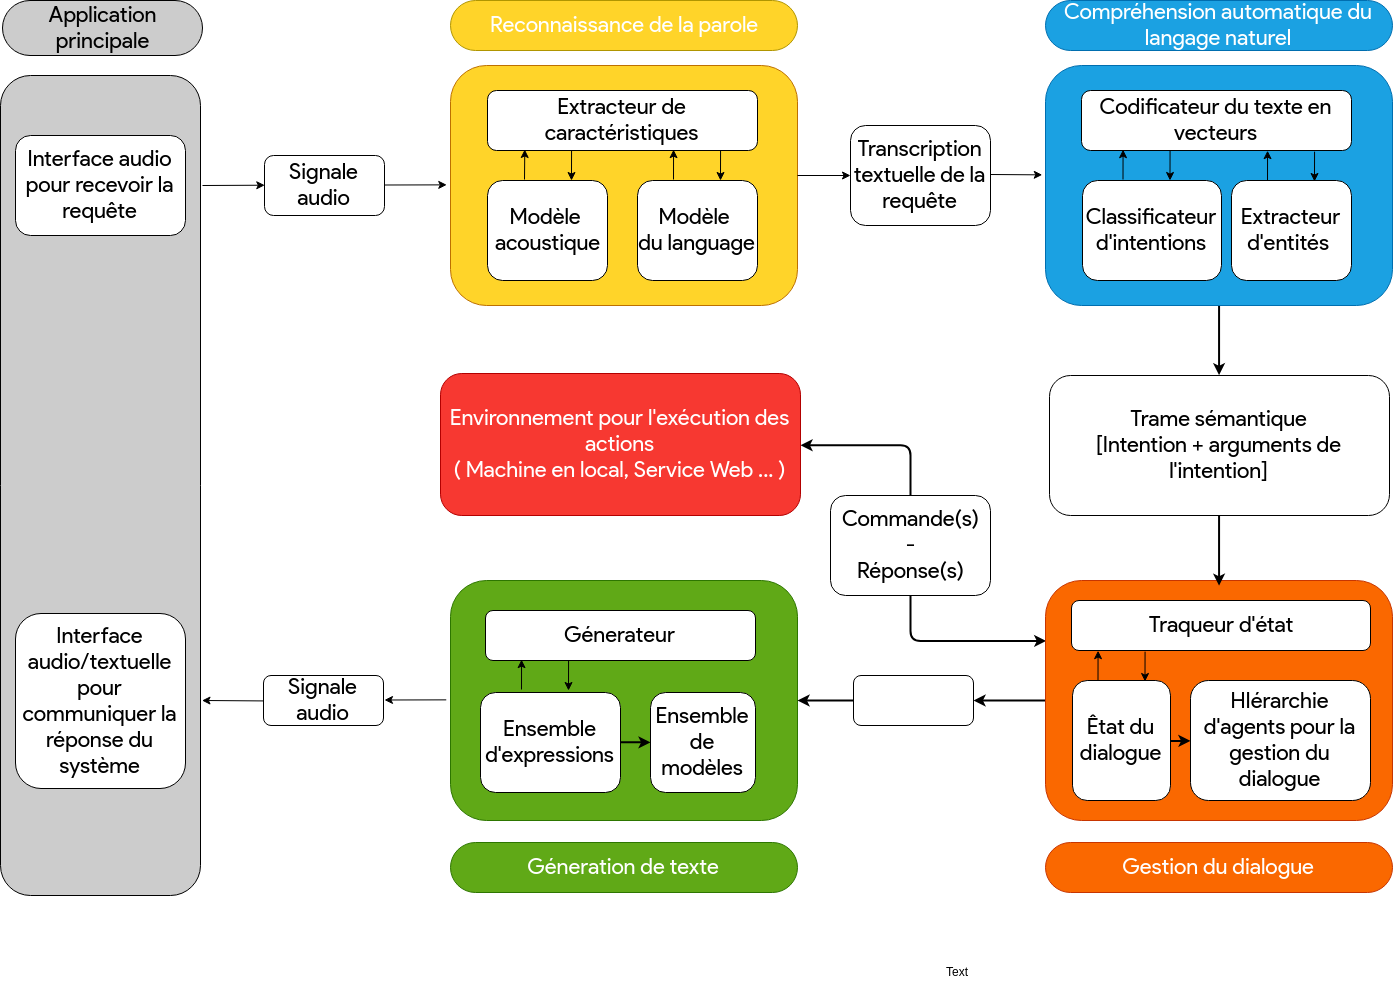
\includegraphics[width=\linewidth]{images/SPA_architecture.png}
	\caption{Architecture haut niveau de Google Assistant \cite{GAlayout}}
\end{figure}
On peut ainsi dégager le schéma simplifié abstrait suivant : 
\begin{figure}[H]
	\centering
	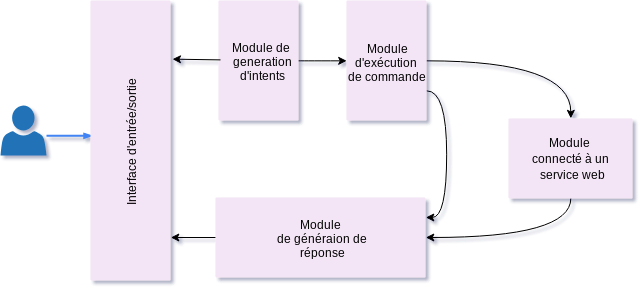
\includegraphics[width=\linewidth]{images/SPA_diagram.png}
	\caption{Architecture abstraite d'un SPA}
\end{figure}


%\section{Points fort des SPAs}
%\paragraph{}
%A travers les sections précédentes ,nous avons appris à découvrir les différents aspect d'un assistants virtuel intelligent, nous avons pu donc apprécié la puissance d'un tel système s'il venait à être perfectionner d'avantage.
%\par En effet, en examinant les domaines d'applications, il est facile de déduire que le recours à un SPA peut grandement faciliter certaines tâches, que ce soit pour celles qui sont les plus triviales et donc peuvent retarder d'autres tâches plus importantes, ou bien celles qui doivent faire appel à la précision ou la grande capacité de calcul des machines, assurant ainsi des résultats précis et rapidement délivrés.
%
\newpage
\section{Conclusion}
\paragraph{}
À travers les sections précédentes, nous avons appris à découvrir les différents aspects d'un assistant virtuel intelligent (caractéristiques, exemples, architectures possibles ...). Nous avons donc pu apprécié la potentielle puissance d'un tel système s'il venait à être perfectionner d'avantage.
\par En effet, en examinant les domaines d'applications, il est facile de déduire que le recours à un SPA peut grandement faciliter certaines tâches, que ce soit celles qui sont les plus triviales pouvant retarder d'autres tâches plus importantes, ou bien celles qui doivent faire appel à la précision et à la grande capacité de calcul des machines, assurant ainsi des résultats précis et rapidement délivrés.
\par
À la fin de ce chapitre nous pouvons donc mettre en valeur la place primordiale que pourrait avoir les SPAs s'ils arrivaient à maturité, c.à.d briser la barrière qui sépare les humains de la machine, parvenant ainsi à faire partie de la vie quotidienne des utilisateurs. 
\par Dans le prochain chapitre nous allons principalement aborder les aspects techniques des différents composants du SPA que nous désirons réaliser.

 


\bibliographystyle{ieeetr}
\bibliography{ref}
\end{document}}

%
%\section{Reconnaissance automatique de la parole}
%
%\subsection{Définition}
%\begin{itemize}
%	\item Définir aussi simplement que possible le processus de RAP(reconnaissance automatique de la parole).
%\end{itemize}
%
%\subsection{Exemples}
%\begin{itemize}
%	\item Donner quelques exemples de système de RAP.
%\end{itemize}
%
%
%\section{Traitement automatique du langage(TAL)}
%
%\subsection{Définition}
%\begin{itemize}
%	\item Petite définition informelle
%\end{itemize}
%
%\subsection{Domaines d'application}
%\begin{itemize}
%	\item Domaines d'applications
%	\item Récentes avancées et découvertes(À VOIR)
%\end{itemize}
%
%\subsection{État de l'art }
%\begin{itemize}
%	\item Récentes avancées et découvertes(À VOIR)
%\end{itemize}
%
%
%\section{Compréhension automatique du langage(CAL)}
%
%\subsection{Définition}
%\begin{itemize}
%	\item Définition aussi formelle que possible en restant bref 
%\end{itemize}
%
%\subsection{Domaines d'application}
%\begin{itemize}
%	\item Domaines d'applications
%\end{itemize}
%
%\subsection{État de l'art }
%\begin{itemize}
%	\item Récentes découvertes et avancées dans le domaine.
%\end{itemize}
%
%
%
%\section{Apprentissage automatique}
%
%\subsection{Définition}
%\begin{itemize}
%	\item  Définir l'apprentissage automatique de manière générale.
%\end{itemize}
%
%\subsection{Domaines d'application}
%\begin{itemize}
%	\item  Définir l'apprentissage automatique de manière générale.
%	\item Paradigmes de l'AA :
%	\begin{itemize}
%		\item Apprentissage génératif
%		\item Apprentissage discriminatif
%		\item Apprentissage profond
%		\item Apprentissage par renforcement
%		...
%	\end{itemize}
%\end{itemize}
%
%
%\subsection{Paradigmes de l'AA}
%\begin{itemize}
%	\item Apprentissage génératif
%	\item Apprentissage discriminatif
%	\item Apprentissage profond
%	\item Apprentissage par renforcement
%	\item Apprentissage interactif
%	...
%\end{itemize}
